\documentclass[11pt, oneside]{article} 
\usepackage{geometry}
\geometry{letterpaper} 
\usepackage{graphicx}
	
\usepackage{amssymb}
\usepackage{amsmath}
\usepackage{parskip}
\usepackage{color}
\usepackage{hyperref}

\graphicspath{{/Users/telliott_admin/Tex/png/}}

\title{Introduction to Kepler}
\date{}

\begin{document}
\maketitle
\Large

\begin{center} 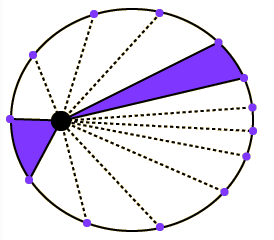
\includegraphics [scale=0.6] {equal_areas.png} \end{center}
This is the first of several chapters in which we work through how Kepler's Laws for the orbits of the planets can be derived from Newton's Laws, namely 
\[ \mathbf{F} = m \mathbf{a} \]

and the inverse square law of gravitation.  
\[ \mathbf{F} = -\frac{GMm}{r^2} \hat{\mathbf{u}}  \]

Kepler's Laws are:  first (K1), the orbits of the planets are not circles but ellipses (non-recurrent orbits may be hyperbolic);  second (K2), the area or arc "swept out" per unit time is the same no matter where in the orbit the planet is;  and third (K3) the period of the orbit is independent of the mass of the planet and its square is proportional to the cube of the length of the semi-major axis of the ellipse.

I also spent some time working on Newton's version of the proof as presented in the \emph{Principia} (see Bressoud's vector calculus book), but he leaves out too many steps.  There is also a version "cooked up" by Richard Feynman and discussed in a book called \emph{Feynman's Lost Lecture}.  

I never got either of these figured out, but if you want to go this route I recommend starting with Feynman.

For myself, I found that once I cleared up a couple of subtleties,  and verified the application of the product rule for differentiation to vector cross-products, it was pretty easy.

\subsection*{circular approximation}
The equation of an ellipse in $xy$-coordinates is 
\[ \frac{x^2}{a^2} + \frac{y^2}{b^2} = 1 \]
where $a$ is one-half the "diameter" in the long dimension and $b$ is one-half the length perpendicular to that.

A second way is to give the focal length, the distance of each of the two foci from the center of the ellipse
\[ f = \sqrt{a^2 - b^2} \]
Yet another way is to give the \emph{eccentricity}, $e$, where 
\[ ea = f  \]

Here is a table of planetary eccentricities I found on the web.

\begin{center} 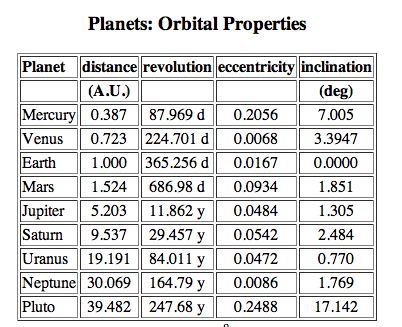
\includegraphics [scale=0.75] {eplanets.png} \end{center}
Mars is the planet that showed Kepler most clearly that the orbits are not circles, but its eccentricity is only 0.09.  For Earth this value is only $0.017$ which gives a focal length of roughly
\[ 0.0167 \times 149.6 \times 10^6 \ \text{km} \approx 2.5 \times 10^6 \ \text{km} \]
which is about $3.5$ times the radius of the Sun.

Next, we look at the geometric proof of K2 used by Newton.
\begin{center} 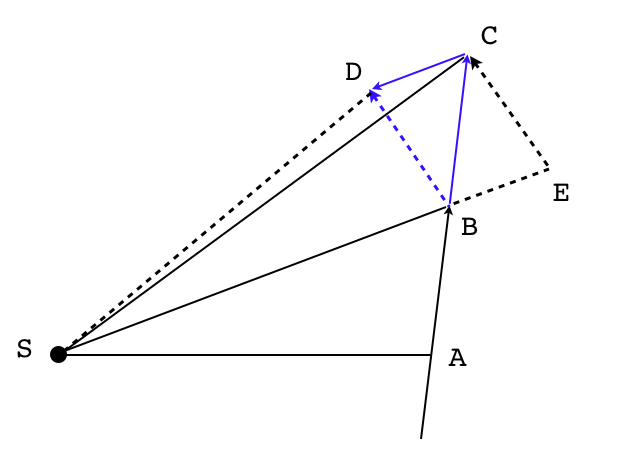
\includegraphics [scale=0.5] {newton_area.png} \end{center}
We diagram the sun $S$ and a planet at $A$.  Imagine that the force toward the sun is applied discretely.  That is, for a small interval $\Delta t$, the planet travels from $A$ to $B$ at constant velocity and if undisturbed, would travel to $C$ in the next unit of time.  

In the absence of a force, the velocity would be constant and so the length of $AB$ is the same as that of $BC$, and since $AB$ is on the same line as $BC$, the area of $\triangle ABS$ is equal to the area of $\triangle BCS$.  

Proof:  draw the vertical line from $S$ to the line containing $ABC$.  The area of either triangle is one-half the length of that altitude times the distance, either $AB$ or $BC$.  The principle is illustrated in the next figure.
\begin{center} 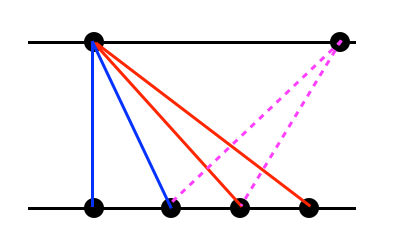
\includegraphics [scale=0.5] {triangles_parallel.png} \end{center}
Given two parallel lines separated by a distance $h$, pick two points on one line separated by a distance $d$ and \emph{any} point on the other line.  The triangles drawn using those points will all have equal area, namely $(1/2)dh$.

Now, suppose the force is applied at $B$ \emph{toward the sun} along $EBS$.  As a result, the trajectory $BC$ is modified by the change in velocity resulting from application of the force toward the sun. The new path is the additional velocity times $\Delta t$.  Call the length $CD$ and add it to $BC$ to give the actual trajectory, $BD$.  

\begin{center} 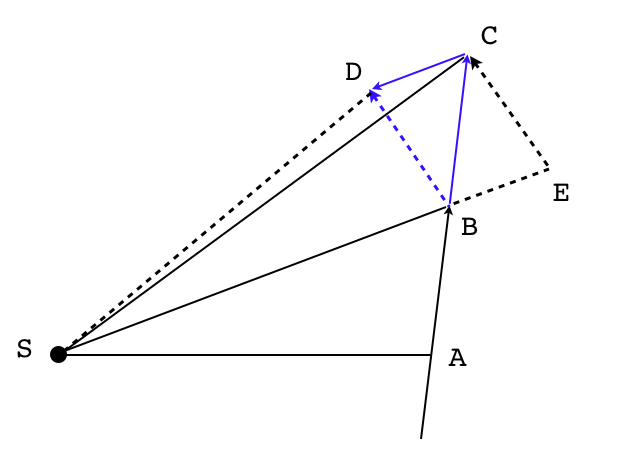
\includegraphics [scale=0.5] {newton_area.png} \end{center}

$CD$ is parallel to $SBE$.  Therefore, every point on $CD$ has the same altitude to $SBE$.  So any point on $CD$ in a triangle with the same base $SB$ will have the equal area no matter which point is chosen.

The area of $\triangle BDS$ is thus equal to the area of $\triangle BCS$, which was found earlier to be equal to the area of $\triangle ABS$.  Since the two triangles from the two intervals of motion have the same area, the area is constant.

\subsection*{Feynman}

Richard Feynman gave a famous series of talks at Cornell in 1964 that were videotaped and transcribed into a book.  Bill Gates later purchased them and put them on the web, unfortunately with some Microsoft DRM.  Still, I have the original book, called \emph{The Character of Physical Law}.  This argument is from Chapter 2, \emph{The Relation of Mathematics to Physics}.

It depends on a tiny bit of calculus---specifically, the product rule for differentiation.  It also uses the fact that the product rule is valid for vector cross products.  (See \hyperref[sec:Vector_cross_product]{\textbf{here}} for a proof).

The rule is that if we have two vectors $\mathbf{a}$ and $\mathbf{b}$ which are functions of time, then
\[ \frac{d}{dt} \ (\mathbf{a} \times \mathbf{b}) = \frac{d\mathbf{a}}{dt} \times \mathbf{b} + \mathbf{a}  \times \frac{d\mathbf{b}}{dt}    \]
In our application the two vectors are the position vector of the planet with respect to the sun, $\mathbf{r}$, and the velocity, which is the time-derivative of that vector.
\[ \frac{d\mathbf{r}}{dt} = \mathbf{v} \]
Or, as the physicists would write it, using Newton's dot notation for the time-derivative:
\[ \mathbf{v} = \dot{\mathbf{r}} \]
We are interested in the area of the triangle formed by the vectors $\mathbf{r}$ and $\dot{\mathbf{r}}$ over a small interval of time.  The area swept out is constant, as Newton showed, and we will prove again here.

A nice feature of the vector cross-product is that it provides (twice) this area.  Namely
\[ A =  \mathbf{r} \times \dot{\mathbf{r}} = |\mathbf{r}| |\dot{\mathbf{r}}| \sin \theta   \]
where $\theta$ is the angle between $\mathbf{r}$ and $\dot{\mathbf{r}}$, and $A$ is the little bit of area.

Our hypothesis is that $A$ is the same no matter where the planet is in its orbit.  Another way to say the same thing is that A doesn't change with time
\[ \frac{d}{dt} \ A = \dot A = 0 \]
Now 
\[ A = \mathbf{r} \times \dot{\mathbf{r}} \]
and we want to compute $\dot A$.  Using the product rule it's easy.
\[ \dot A = \frac{d}{dt} \ (\mathbf{r} \times \dot{\mathbf{r}}) \]
\[ \dot A = \dot{\mathbf{r}} \times \dot{\mathbf{r}} \ + \ \mathbf{r} \times \ddot{\mathbf{r}} \]
As Feynman says: it's just playing with dots.  

Let's look at those two terms.

A nice fact about the cross-product is that if the two vectors point in the same direction, then the cross-product is zero.  Any vector points in the same direction as itself, so the first term is certainly zero.  
\[ \dot{\mathbf{r}} \times \dot{\mathbf{r}} \ = 0 \]
Next, recall that the second derivative with respect to time of the position is the acceleration vector.  According to Newton's second law, the force of gravity points toward the sun, radially.  

But of course the position vector also points out radially from the sun.  $\mathbf{r}$ and $\ddot{\mathbf{r}}$ are in the same direction (the opposite direction \emph{is} the same direction, multiplied by $-1$), so the cross-product is again zero.
\[ \mathbf{r} \times \ddot{\mathbf{r}} \ = 0 \]
So that means the whole thing is zero.
\[ \dot A = \dot{\mathbf{r}} \times \dot{\mathbf{r}} \ + \ \mathbf{r} \times \ddot{\mathbf{r}} = 0 + 0 = 0  \]

We have shown that the time-derivative of the area is zero, so the area is constant, which is Kepler's second law.

\end{document}  